\documentclass[t]{beamer}
\usetheme{Copenhagen}
\setbeamertemplate{headline}{} % remove toc from headers
\beamertemplatenavigationsymbolsempty

\usepackage{amsmath, array, tikz, bm, pgfplots, tcolorbox, graphicx, venndiagram, color, colortbl}
\pgfplotsset{compat = 1.16}
\usepgfplotslibrary{statistics}
\usetikzlibrary{trees}

\title{Overview of Statistics}
\author{}
\date{}

\AtBeginSection[]
{
  \begin{frame}
    \frametitle{Objectives}
    \tableofcontents[currentsection]
  \end{frame}
}

\begin{document}

\begin{frame} 
\maketitle
\end{frame}

\section{Identify the population and a sample}

\begin{frame}{What is Statistics?}
\begin{tcolorbox}[colframe=green!20!black, colback = green!30!white,title=\textbf{Statistics}]
\textbf{Statistics} is the process of obtaining, organizing, summarizing, interpreting, and drawing conclusions based on observable values called \textit{data}.
\end{tcolorbox}
\vspace{10pt}	\pause

Typically, statisticians gather samples of data to help draw conclusions about the data's population.
\end{frame}

\begin{frame}{Population and Sample}
\begin{tcolorbox}[colframe=green!20!black, colback = green!30!white,title=\textbf{Population}]
The \textbf{population} is composed of all entities (\textit{data values}) to be observed. The information we obtain from a population is referred to as a \textbf{parameter}.
\end{tcolorbox}
\vspace{6pt}	\pause
\begin{tcolorbox}[colframe=green!20!black, colback = green!30!white,title=\textbf{Sample}]
The \textbf{sample} is a subgroup (a.k.a. \textit{subset}) of the population. The information we obtain from a sample is referred to as a \textbf{statistic}.
\end{tcolorbox}
\vspace{6pt}	\pause
A sample drawn from a population should be a good representation of that population, and should be big enough to include a variety of observations.
\end{frame}

\begin{frame}{Population vs. Sample Visual Interpretation}
\begin{center}
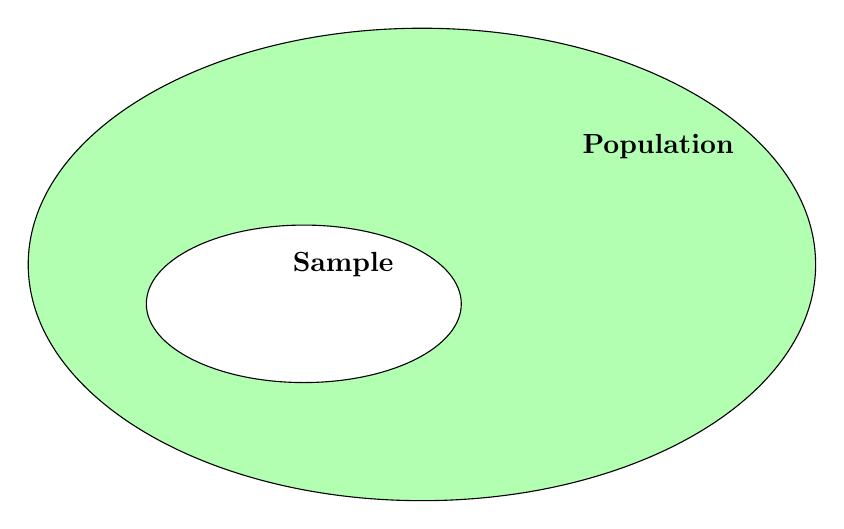
\begin{tikzpicture}
\draw [fill=green!30] (0,0) ellipse (5cm and 3cm);
\node at (3,1.5) {\textbf{Population}};
\draw [fill=white] (-1.5,-0.5) ellipse (2cm and 1cm);
\node at (-1,0) {\textbf{Sample}};
\end{tikzpicture}
\end{center}
\end{frame}

\begin{frame}{Example 1}
Identify the population and the sample of each of the following.	\newline\\
(a)	\quad 100 people at the mall were surveyed as to whether or not they like the mall. \newline\\	\pause
Population: Everyone at the mall. \pause	\newline Sample: The 100 people surveyed	\newline\\	\pause
(b)	\quad Doctors analyzed the MRIs of 38 professional boxers for possible brain injury.	\newline\\	\pause
Population: All professional boxers \pause	\newline Sample: The 38 professional boxers
\end{frame}

\section{Distinguish between statistical and practical significance}

\begin{frame}{Statistical Significance}
As we progress, keep in mind that chance and randomness are always a factor in the study of statistics, and things are not as foolproof as they are in other math courses.	\newline\\	\pause

A big part of interpreting and drawing conclusions from statistical results is to determine if they are considered statistically significant.	\newline\\	\pause


\begin{tcolorbox}[colframe=green!20!black, colback = green!30!white,title=\textbf{Statistically Significant}]
\textbf{Statistically significant} results are those that are not likely obtained by chance.
\end{tcolorbox}
\end{frame}

\begin{frame}{Example 2}
Determine if each outcome would be considered statistically significant.	\newline\\
(a)	\quad Flipping a coin 100 times and getting tails 94 times.	\newline\\	\pause
Since this result is very unlikely to happen by chance, it is considered statistically significant.	\newline\\	\pause
(b)	\quad Flipping a coin 100 times and getting tails 53 times.	\newline\\	\pause
Since we expect the coin to come up heads roughly half the time and tails the other half, this result is not considered statistically significant.
\end{frame}

\begin{frame}{Practically Significant}
\begin{tcolorbox}[colframe=green!20!black, colback = green!30!white,title=\textbf{Practically Significant}]
\textbf{Practically significant} results are those that are useful in the real world.
\end{tcolorbox}
\vspace{8pt}	\pause

For instance, an SAT prep course might have statistically significant results (e.g. a high percentage of people did improve their scores), but if the improvement is small, such as 20 points, the results might not be practical enough to purchase it.
\end{frame}

\end{document}